% $Id: $
\documentclass[a4paper, 10pt]{article}
% reduced margins
\usepackage{fullpage}
\usepackage[authoryear]{natbib}
% spacing
\usepackage{setspace}
% page headings
\usepackage{fancyhdr}
%\usepackage{lscape}

%\usepackage[nomain,acronym,xindy,toc]{glossaries} % nomain, if you define glossaries in a file, and you use \include{INP-00-glossary}
%\makeglossaries

\usepackage[margin=1.0in]{geometry}
\usepackage{url, subeqn, multirow}
\usepackage{booktabs}
\usepackage{enumerate}

\setlength{\headheight}{15.2pt}
\pagestyle{fancy}
% urls

\usepackage{lscape}
\usepackage{graphicx}
\usepackage{color}
\usepackage{hyperref}
\usepackage{url}
\hypersetup{colorlinks, urlcolor=darkblue}
\usepackage{pdfpages}

\usepackage{lscape}
% figs to be 75% of test width
\setkeys{Gin}{width=0.75\textwidth}

\usepackage{color}
\newcommand{\laurie}{\textcolor{blue}}
\newcommand{\coilin}{\textcolor{green}}


\title{Supply of Research Services to establish MSY proxies for data-limited stocks (2017-18) to the Marine Institute, Rinville, Oranmore, Co. Galway.
(Ref: ITT17-015)}

\author{Laurence Kell, C\'oil\'in Minto}
\date{\today}

\pdfinfo{%
  /Title    (MSY reference points for data-limited stocks)
  /Author   (Laurence Kell)
  /Creator  ()
  /Producer ()
  /Subject  ()
  /Keywords ()
}


%
\renewcommand{\abstractname}{\large SUMMARY}
%
\newcommand{\Keywords}[1]{\begin{center}\par\noindent{{\em KEYWORDS\/}: #1}\end{center}}
%
\makeatletter
\renewcommand{\subsubsection}{\@startsection{subsubsection}{3}{\z@}%
  {-1.25ex\@plus -1ex \@minus -.2ex}%
  {1.5ex \@plus .2ex}%
  {\normalfont\slshape}}
\renewcommand{\subsection}{\@startsection{subsection}{2}{\z@}%
  {-3.25ex\@plus -1ex \@minus -.2ex}%
  {1.5ex \@plus .2ex}%
  {\normalfont\bfseries\slshape}}
\renewcommand{\section}{\@startsection{section}{1}{\z@}%
  {-5.25ex\@plus -1ex \@minus -.2ex}%
  {1.5ex \@plus .2ex}%
  {\normalfont\bfseries}}
\makeatother
%
\renewcommand\thesection{\arabic{section}.}
\renewcommand\thesubsection{\thesection\arabic{subsection}}
\renewcommand\thesubsubsection{\thesubsection\arabic{subsubsection}}
%
\renewcommand{\headrulewidth}{0pt}

\usepackage{listings}

\newenvironment{mylisting}
{\begin{list}{}{\setlength{\leftmargin}{1em}}\item\scriptsize\bfseries}
{\end{list}}

\newenvironment{mytinylisting}
{\begin{list}{}{\setlength{\leftmargin}{1em}}\item\tiny\bfseries}
{\end{list}}

\usepackage{listings}

\definecolor{darkblue}{rgb}{0,0,0.5}
\definecolor{shadecolor}{rgb}{1,1,0.95}
\definecolor{shade}{rgb}{1,1,0.95}


\lstset{ %
language=R,   % the language of the code
basicstyle=\footnotesize, % the size of the fonts that are used for the code
numbers=left,   % where to put the line-numbers
numberstyle=\footnotesize, % the size of the fonts that are used for the line-numbers
stepnumber=1	00,   % the step between two line-numbers. If it's 1, each line 
    % will be numbered
numbersep=5pt,   % how far the line-numbers are from the code
backgroundcolor=\color{shade}, % choose the background color. You must add \usepackage{color}
showspaces=false,  % show spaces adding particular underscores
showstringspaces=false,  % underline spaces within strings
showtabs=false,   % show tabs within strings adding particular underscores
frame=single,   % adds a frame around the code
tabsize=2,   % sets default tabsize to 2 spaces
captionpos=b,   % sets the caption-position to bottom
breaklines=true,  % sets automatic line breaking
breakatwhitespace=false, % sets if automatic breaks should only happen at whitespace
title=\lstname,   % show the filename of files included with \lstinputlisting;
    % also try caption instead of title
escapeinside={\%*}{*)},  % if you want to add a comment within your code
morekeywords={*,...}  % if you want to add more keywords to the set
}


%
\begin{document}

\onehalfspacing
\lhead{\normalsize\textsf{MyDas- Ref: ITT17-015}}
\rhead{}

\maketitle
% gets headers on title page ...
\thispagestyle{fancy}
% ... but not on others
\pagestyle{empty}

%

\newpage
\tableofcontents
\newpage

\begin{abstract}

\textit{
Trends and fluctuations in populations are determined by complex interactions between extrinsic forcing and intrinsic dynamics. For example, stochastic recruitment can induce low‐frequency variability, i.e. ‘cohort resonance’, which can induce apparent trends in abundance and may be common in age‐structured populations; such low‐frequency fluctuations can potentially mimic or cloak critical variation in abundance linked to environmental change, over‐exploitation or other types of anthropogenic forcing (Bjørnstad, 2004). Although important, these effects can be difficult to disentangle. The simulations so far show that life histories are important and should be used to help condition operating models to ensure robust feedback-control rules. MSE is important to help develop these robust feedback control rules and to help identify appropriate observational systems.
Although the performance of the HCR depended on the life-history characteristic, it was not in the way initially expected, i.e. the outcomes could not be grouped solely by whether the Operating Models (OMs) represented fast growing vs. late maturing species or demersal vs. pelagic stocks. What was important was the nature of the dynamics, i.e. how variable was the stock between years; for example, a stock could exhibit high interannual variability if natural mortality and recruitment variability was high, regardless of the values of k, Linf, L50. The nature of the indices is also important; for example, even if a stock had low interannual variability, an index could be highly variable if it was based on juveniles or there were large changes in spatial distribution between years. It is therefore necessary to look at the robustness of HCRs to the nature of the time-series of the stock (as represented by the OM) and to the characteristics of the data collected from it (as represented by the Observation Error Model). This will require tuning by constructing a reference set of OMs and then tuning the HCR to secure the desired trade-offs. The work so far can be considered as focusing first on developing HCR that perform satisfactorily for a reference set, the next step is to develop case-specific HCRs.


\begin{enumerate}[8]

\item Aspects to consider for the 3.2.1 rule by the next meeting would be:

\begin{enumerate}[8.1]

\item Investigating the impact of relative weighting of the r, f and b components of the rule on the performance of the rule;

\item Investigating more extensively the time-lag properties of the r component, including alternative formulations;

\item Setting of appropriate reference levels in the f and b component of the rules, and the extent to which this could be done with tuning that depends on life-history traits and/or the nature of the time-series;

\item Investigation of the use of trends in an index without a reference level.

\end{enumerate}

\item Longer term aspect to consider for data-limited rules:

\begin{enumerate}[9.1]

\item Focusing on the nature of time-series and developing diagnostics that could help determine the rules that would work well under alternative characterisations of the nature of the time-series, and aspects such as quality of data used by the rules (and hence ability to detect signals), ability to set appropriate reference points, etc.;

\item Linking life-history traits, the form of density-dependence and fishery characteristics (e.g. including fishery selectivity) to the nature of resulting time-series;

\item Develop guidance for use of catch rules by linking (a) and (b);

\item Avoiding the shot-gun approach to simulation testing e.g. by making more extensive use of sensitivity (elasticity) analysis to highlight factors that are most important in determining the time-series behaviour of stocks;

\item Investigating the implications of how the operating models are set up (fishing history, depletion levels, selectivity assumptions, mortality) on the behaviour of the stock and on the performance of the catch rule.

\end{enumerate}

}

\end{abstract}

\onehalfspacing
\lhead{\normalsize\textsf{SCRS/2014/025}}
\rhead{}

\maketitle
% gets headers on title page ...
\thispagestyle{fancy}
% ... but not on others
\pagestyle{empty}


\maketitle

\newpage\section{The Call}

The overall aim of the project is to develop and test a range of assessment models and methods to establish MSY reference points (or proxy MSY reference points) across the spectrum of data-limited stocks. There is a requirement for the following research services over a 24 months period between May 2017 and April 2019: 

\begin{description}
 \item[Task 1:] \textbf{\textit{Stock prioritisation}} A number of example stocks have been identified (\textbf{Table \ref{tab:stocks}}). The final list of stocks will be prioritised using criteria like: economic value of the stock; importance of the species to the ecosystem (key-stone species); sensitivity to the impacts of fishing; available data. 
 \item[Task 2:] \textbf{\textit{Data collation}} To run in parallel with other tasks. The project relies on existing data sets, however these data need to be collated in a usable form. Most datasets are available from the Marine Institute, or are publicly available, but others may only exist in other European labs/agencies. 
 \item[Task 3:] \textbf{\textit{Method and simulation framework development and implementation}} A number of data-limited methods exist. In order to compare the performance of these methods it would be useful to implement them all in the same framework, e.g. R. New methods may also be developed in the same framework. 
 \item[Task 4:] \textbf{\textit{Method performance appraisal}} Develop a set of diagnostics that can be applied across range of models. Also assess the stability of the model, sensitivity to assumptions and bias in the advised catch. 
 \item[Task 5:] \textbf{\textit{Reference point comparisons}} Once reference points have been identified, their performance should be evaluated through simple management strategy evaluations. 
 \item[Task 6:] \textbf{\textit{Liaison with Marine Institute}} The service provider is expected to meet on a regular basis with Marine Institute staff involved in the project: Monthly update meetings at the Marine Institute premises in Oranmore Galway 
 %\item[Task 7:] \textbf{\textit{Linkage with other projects}} CPV codes 71354500-9 Marine survey services 73112000-0 Marine research services 90712300-4 Marine conservation strategy planning 98360000-4 Marine services 77700000-7 Services incidental to fishing 73000000-2 Research and development services and related consultancy services 73110000-6 Research services 73200000-4 Research and development consultancy services 73210000-7 Research consultancy services. \\
 %Monkfish MSE (MI-GMIT Cullen fellowship); Newport Research Cluster Project, Marine Research Programme (Unlocking the Archive project; MI-GMIT); DGMARE Tender: Study on approaches to management for data-poor stocks in mixed fisheries (DRuMFISH) (GMIT partner in consortium); Conservation International-FAO (Global Status of Data-Poor Stocks). 
 \item[Task 7:] \textbf{\textit{Linkage with other projects}} The service provider is required to link research output to the following projects: 
 \begin{itemize}
  \item The International Council of the Exploration of the Sea (ICES) is in the process of developing methods to identify MSY proxy reference points for data-limited stocks (WKLIFE and WKPROXY series of workshops). The service provider is required to contribute to this process by proposing and testing new assessment models and methods of establishing reference points and will be expected to attend up to 4 one-week meetings at ICES headquarters in Copenhagen. However there are key differences with the ICES approach: \\
This research contract will include stocks not currently assessed by ICES;
this research contract will focus on the available data for each stock first and on the methods second; the ICES approach focuses on the methods first and then applies a limited number of methods to a large number of stocks.
\item Marine Institute research and development on data poor stocks which includes the biology, stock dynamics and Management Strategy Evaluation (MSE) for Pollock.  It is expected that the service provider will collaborate closely with the team developing assessment methods for the pollock stock.
\item Galway Mayo Institute of Technology GMIT had been awarded a Cullen fellowship for a PhD project on management strategy evaluation for monkfish. It is expected that the Cullen PhD and service provider will closely collaborate on tasks like data collation, assessment model implementation, simulation model development and management strategy evaluation. 
\end{itemize}
\end{description}


\section{Project Plan}
%\newpage\section{Our Proposal}
The principles of the European Union Common Fisheries Policy (CFP), which has driven the management of Europe's common fisheries resources since 1983, are to manage the activities of fishing fleets aims to ensure sustainable exploitation of the ocean's living resources, the provision of important food resources to humankind, and the profitability of an industry that is an important economic and social activity in many areas of Europe and elsewhere. The overall aim of the project is to support the CFP by developing and testing a range of assessment models and methods to establish MSY reference points (or proxy MSY reference points) across the spectrum of data-limited stocks. 

Quantitative scientific advice is at the heart of fisheries management regulations, providing estimates of the likely current and future status of fish stocks through statistical population models, termed stock assessments, but also probabilistic comparisons of the expected effects of alternative management procedures. Management Strategy Evaluation (MSE) uses stochastic simulation to incorporate both the inherent variability of natural systems, and our limited ability to model their dynamics, into analyses of the expected effects of a given management intervention on the sustainability of both fish stocks and fleets.

Following the adoption of the precautionary approach \citep[PA,][]{garcia1996precautionary} by many fisheries organisations, biological reference points have become central to management. Reference points are used as targets to maximise surplus production and limits to minimise the risk of depleting a resource to a level where productivity may be compromised. They must integrate biological processes such as growth, recruitment, mortality and connectivity into indices for productivity and spawning reproductive potential \citep{kell2015spawning} to provide limits and targets for exploitation. They are increasingly required for by-caught, threatened, endangered, and protected species where data and knowledge are limited, not just for the main commercial stocks, where analytical assessments are available \citep{sainsbury2003ref}.

A main objective of reference points is to prevent overfishing, e.g. growth, recruitment, economic and target overfishing. Growth and recruitment overfishing are generally associated with limit reference points, while economic overfishing may be expressed in terms of either targets or limits. The difference between targets and limits is that indicators may fluctuate around targets but in general limits should not be crossed. Target overfishing occurs when a target is overshot, although variations around a target is not necessarily considered serious unless a consistent bias becomes apparent. In contrast even a single violation of a limit reference point may indicate the need for immediate action. Therefore to achieve MSY requires limit as well as target reference points.

\newpage\subsection{Workplan}

A variety of reference points and methods for deriving them are used for both data rich and poor stocks. In a data rich situtation reference points may be derived directly from a stock assessment model, e.g. in a biomass dynamic model where MSY is a function of the estimated parameters ($r$ and $K$); ad-hoc approaches when using age methods such as Virtual Ppopulation Analysis, where assumptions about the stock recruitment relationship and future selection and biological parameters have to be made after fitting the assessment model; or in a state space formulation \citep{nielsen2014estimation} which actually estimates a prediction mechanism and reference points. 

In data poor situations a wide variety of statistical methods have been used or proposed to estimate stock status, productivity, fishing rates and reference points, for example using samples of length-composition  \citep{kokkalis2015limits,prince2015length}, age-composition  \citep{thorson2015catch}, fishery catch and fishing effort data  \citep{roa2015hierarchical}, abundance indices  \citep{needle2015using} or simple length-based reference points  \citep{cope2009length}. Before  being able to make management recommendations, a link between a trigger reference point and stock status has to be identified, e.g. so a harvest control rule (HCR) can be used to link removals to the current state of the resource  \citep{restrepo1999precautionary}. \cite{cope2009length} proposed a way to do this for catch-based length indicators, using a decision tree and a risk assessment. This approach could be used for a range of indicators. However, \citep{cope2009length} also noted that a full examination of such an approach requires a management strategy evaluation.  

In an MSE setting reference points are tuned (i.e. chosen) to meet management objectives. Harvest strategies (i.e. HCRs) can either be model based or empirical \cite{dowling2015empirical}, in the former a stock assessment is used to estimate stock status and reference points while in the later management is based on trends in the data directly. The Commission for the Conservation of Southern Bluefin Tuna (CCSBT) provides a model-free example of a MP \citep{hillary2015scientific} that is based on year-to-year changes and trends in empirical indicators (i.e. CPUE and fisheries independent indices); reference levels are then tuned to meet management objectives using MSE, where tuning refers to adjusting the parameters of the MP to try and achieve the stated objectives represented by the OM. Model-based MPs, for example those based on a stock assessment model, may include the estimation of MSY-based reference points, but the values of F, $F_{MSY}$ , B and $B_{MSY}$ from the OM do not need to be equivalent to their proxies in the MP (e.g. if a stock assessment models used in the MP is structually different from that used to condition the OM).

WKLIFE was tasked with developing operational methods for setting proxy reference points for stocks where survey based assessments indicate trends (category 3) and for which reliable catch data are available (category 4). Methods so far examined include length-based indicators, spawning potential ratio (SPR), catch and cpue, and catch only based methods. These methods are now being implemented by the ICES study group WKPROXY, and along with others \citep[][]{thorson2015introduction, carruthers2014evaluating}, will be first evaluated using simulation, e.g. using crosstesting where a data rich stock assessment is used to generate data and then fitted to a data poor model and estimates of stock status compared. This approach requires a data rich assessment and that the stock assessment represents the stock dynamics. Alternatively life history theory and relationships can be used to simulate stocks and fisheries for a variety of hypotheses about their dynamics, i.e. using the FLife package \citep[see][]{rosenberg2014developing}.
To ensure a management advice framework based on a stock assessment and reference points (i.e. a control system) is robust requires showing that it still functions correctly in the presence of uncertainty or stressful environmental conditions \citep{radatz1990ieee}. This requires an Operating Model (OM, i.e. a simulation model that represents hypotheses about resource dynamics) conditioned on ecological processes that affect the behaviour of management systems, i.e the focus is on the future, not on fitting historical data as when conditioning an OM on a stock assessment. This is a less data, and more hypothesis-orientated approach \citep{kell2006operational}. 

To conduct MSE requires six steps \citep{punt2007developing}; namely

  \begin{description}%[<+->]
    \item[Identification] of management objectives and mapping these to performance measures to quantify how well they are achieved\
    \item[Selection] of hypotheses about system dynamics for building \textbf{O}perating \textbf{M}odels (i.e. Simulation Models)
    \item[Building] the simulation models, i.e. conditioning them on data and knowledge, and rejecting and weighting different hypotheses.
    \item[Identifying] alternative management strategies, (i.e.the combination of pre-defined data, stock assessment methods, reference points and HCRs.
    \item[Running] the simulations using the HCRs as feedback control procedures; and
    \item[Agreeing] the Management Strategies that best meet management objectives.
 \end{description}

The MSE will be conducted using FLR\footnote{http://www.flr-project.org/} \citep{kell2007flr} a family of packages in R for conducting MSE and stock, following the tasks below.
Task 1 will help identify stocks and management objectives; Task 2 will allow the OMs to be conditioned; Task 3 will allow the OM to be implemented and psuedo data simulated to evaluate the proposed stock assessment methods and reference points; Task 4 will screen the candidate stock assessment methods (both those considered by WKLIFE but others to ensure that methods are state-of-the-art); and Task 5 will conduct MSE. Task 6 will ensure that the project delivers tools that make a major contribution to the management of data poor stocks; and Task 7 will help in dissemination, and ensure that methods developed tested across a wide range of case studies. 

\newpage\subsection{Tasks}

\subsubsection{Task 1: Stock prioritisation (\laurie{Laurie})}

\textit{\textbf{A number of example stocks have been identified. The final list of stocks will be prioritised using criteria like: economic value of the stock; importance of the species to the ecosystem (key-stone species); sensitivity to the impacts of fishing; available data.}}

The final choice of stock will be made after the award of the contract based on their economic, social and ecological importance but also to reflect a contrasting range of life histories, fisheries and datasets. We will however focus on the following stocks:

\begin{itemize}
 \item Sprat in the Celtic Sea and West of Scotland Sprat (Sub-area VI \& Divisions VIIa-c and f-k)
 \item Grey gurnard VI \& VII (excl. VIId)
 \item Ling IIIa, IVa, VI, VII, VIII, IX, XII, and XIV 
 \item Rays, primarily in areas VIIa,f,g 
 \item John dory in ICES Sub-area VII and Divisions VIIIa,b and d (Northeast Atlantic)
 \item In collaboration with Newport STO:
\begin{itemize} 
 \item Saithe VII, VIII, IX, X
 \item Pollock VII
\end{itemize}
\item Turbot VIIe,f,j,h and sub area VIII and IXa
\item Brill VII (or suitably defined)
\end{itemize}
A meta-database will be created identifying the data sources and relevant publications for the potential stocks of interest but also for related stocks and species. A reason for considering related stocks and species is because it is possible to compare the performance of data poor and data rich methods using cross-testing. In a cross-test data and population estimates from a data rich assessment are used to simulate data poor datasets which can then be used to test data poor assessment methods, allowing candidate methods to be identified. While a Robin Hood approach can be used to take information from data rich stock to inform assessments of information poor species, i.e. taking from the rich to help the poor. Since similarities in taxonomy, life-history or ecology allows the information from ‘data-rich’ stocks to be utilised as ‘prior distributions’ or penalty functions for the data poor species. Hierarchical Bayesian methods allow poor-data species to borrow strength from species with good-quality data. \cite{jiao2011poor} for example used hierarchical Bayesian state-space surplus production models and showed estimates were considerably more robust than those of the nonhierarchical models.

Once the meta-database has been prepared (end of month 1) then a list of study stocks will be agreed, following which a database will be designed and an attempt to aquire the data made, following which the final list will be agreed (end of month 2). 


\subsubsection{Task 2: Data collation (\laurie{Laurie})}

\textit{\textbf{Data collation (to run in parallel with other tasks) The project relies on existing data sets, however these data need to be collated in a usable form. Most datasets are available from the Marine Institute, or are publicly available, but others may only exist in other European labs/agencies.}}

Datasets will include, stock assesment datasets (ICES, NAFO, STECF\footnote{https://stecf.jrc.ec.europa.eu/dd/medbs/ram}, ...), fisheries, life history parameters (Fishbase\footnote{http://www.fishbase.org/search.php}, fishnets\footnote{https://github.com/fishnets/fishnets}), surveys (MI), commercial sampling sets (MI), and economic data (e.g. BIM).

Life history data will also be compiled since many studies have shown the relationships between life history traits for processes such as growth, maturity and natural mortality. Life history has also been used to develop priors in stock assesments for difficult to estimate parameters. e.g. the population growth rate (r) in data poor assessments. Life history parameters can also be used to develop an Operating Model.

The meta-database will be extended with code to read the data into a common format, e.g. data frames and other objects in R and FLR to model stocks, populations and fisheries. It is important to ensure that data are easily available and that any processing steps are well documented and standardised this is true for both the basic data and the results from the MSE (e.g. datasharing\footnote{https://github.com/AdrianHordyk/datasharing}).
s.


\subsubsection{Task 3: Framework Development (\laurie{Laurie})}

\textit{\textbf{Method and simulation framework development and implementation A number of data-limited methods exist. In order to compare the performance of these methods it would be useful to implement them all in the same framework, e.g. R. New methods may also be developed in the same framework.}}

All methods will be implemented in R and be compatible with The Fishery Library in R (\textbf{FLR})  \citep{kell2007flr}, a project that has for the last ten years been building an extensible toolset of statistical and simulation methods for quantitative fisheries science, with the overarching objective of enabling fisheries scientists to carry out analyses of management procedures in a simplified and robust manner through the MSE approach.

\textbf{FLR} has become widely used in many of scientific bodies providing fisheries management advice, both in Europe and elsewhere. The evaluation of the effects of elements of the revised CFP, the analysis of the proposed fisheries management plans for the North Sea, or the comparison of management strategies for Atlantic tuna stocks, among others, have used the \textbf{FLR} tools to advice managers of the possible courses of action to favour the sustainable use of many marine fish stocks.

The \textbf{FLR} toolset is currently composed of a variety of packages, covering the various steps in the fisheries advice and simulation workflow. They include a large number of S4 classes, and more recently Reference Classes, to model the data structures that represent each of the elements in the fisheries system. Class inheritance and method overloading are essential tools that have allowed the \textbf{FLR} packages to interact, complement and enrich each other, while still limiting the number of functions an user needs to be aware of. Methods also exist that make use of R's parallelization facilities and of compiled code to deal with complex computations.

Using \textbf{FLR} means that advantage can be taken of existing methods, and that dissemination and support is easier and will be maintained after the life of the project.  Under the project development will be on mainly on four packages \textbf{FLife}, \textbf{mpb}, \textbf{hcr} and \textbf{oem}. In addition new methods will be added to other \textbf{FLR} packages as appropriate. 

\textbf{FLife} is a package for modelling life history relationships, e.g. for developing priors, estimating quantities such a Z from length data, deriving reference points and indicators and for creating OMs.

\textbf{mpb} is a package for modelling biomass dynamic based management procedures, it has also been used to assess a variety of stocks, e.g. Atlantic bigeye and North Atlantic albacore and swordfish. It also forms the basis of the North Atlantic albacore MP evaulated using MSE.

\textbf{hcr} will be a new package that will include a variety of emprirical HCRs, e.g. those used by CCSBT, proposed by ICES and from a review of the literature \cite[e.g.][]{pomarede2010evaluating}.

\textbf{oem} will be a new package that implements a variety of observation error models, that will be used to simulate a variety of datasets from OMs that will be used by the data poor methods.

In addition Dr Kell is the developer of two packages that are used to provide a common set of diagnostics across stock assessment methods (\textbf{diags}) and to summarise stock status relative to reference points and for summarising the results from MSE (\textbf{kobe})

There are a variety of R packages, that already implement a variety of data poor methods, e.g. https://github.com/quang-huynh/MLZ, https://github.com/AdrianHordyk/LBSPR  https://github.com/cran/DLMtool, wherevever possible these packages will be used and we will collaborate with their developers.


\subsubsection{Task 4: Method Performance Appraisal (\laurie{Laurie})}

\textit{\textbf{Method performance appraisal Develop set of diagnostics that can be applied across range of models. Also assess the stability of the model, sensitivity to assumptions and bias in the advised catch.}}

A range of summary statistics will be required to illustrate trade-offs between multiple potentially conflicting objectives. Although there are many potential summary statistics so that decision makers can choose between tangible options on the basis of actual projections rather than abstract concepts and performance statistics, however,  should ideally be few, informative and based axes such as  ‘stock status’, 'safety', 'stability' and 'yield'. It is also necessary to distinguish between techincal summary statistics (i.e. those required to evaluate model fits and performance) and those required to evaluate management objectives.

Results will be presented using an interactive app, based on shiny, that can be used to evaluate the performance of the models.


\subsubsection{Task 5: Reference Point Comparisons (\laurie{Laurie}, \coilin{C\'oil\'in})}

\textit{\textbf{Reference point comparisons (across candidate methods) Once reference points have been identified, their performance should be evaluated through simple management strategy evaluations.}}
A set of appropriate stock assessment models will be fit to the available data (Task 1 and 2). Methods used will reflect the available data on a stock-by-stock basis (Task 2) and also methods available or developed in Tasks 3 and 4. Performance diagnostics (e.g., residual inspection, retrospective patterns) will be run for each assessment model fit.\\
We will provide a review of reference points and indicators, based on a variety of assumptions, e.g. MSY based on biomass dynamic stock assessment models, and indicators such as $L_{opt}$,$L_{50}$ and $L_{mega}$ for length-based methods. Then compare these using simulation, e.g. cross-testing and simulations based on FLife. This will allow the power of the methods to detect whether a stock has achieved its targets and avoid its limits. Based on this screening process a set of candidate reference points and assessment methods will be proposed for MSE.

MSE will include a Value-of-infomation analysis, where the benefits of collecting better data and new infomation will be evaluated.

\subsubsection{Task 6: Liaison with Marine Institute (\coilin{C\'oil\'in}, \laurie{Laurie}, \laurie{Laurie})}

\textit{\textbf{The service provider is expected to meet on a regular basis with Marine Institute staff involved in the project:  Monthly update meetings at the Marine Institute premises in Oranmore Galway}}

The proposal is ambitious but achievable. However there needs to be good communication between the consortum and the Marine Instiutute to ensure the project keeps focused and delivers. Therefore we will arrange monthly face-to-face meetings, make all code, data and results available on the cloud and in a suitable repository (e.g. github) and provide a web based interface for model results.\\
Wider project 6-monthly progress reports and meetings at the Marine Institute will ensure the over-arching goals of the project are achieved.

\subsubsection{Task 7:  Linkage with other Projects (\coilin{C\'oil\'in})}

 \begin{itemize}
  \item Monkfish\\
  This project will develop in close collaboration with the Cullen Fellowship of Mr Luke Batts, co-supervised by Dr Hans Gerritsen (MI) and Dr C\'oil\'in Minto (GMIT). Active collaboration will occur with Tasks 3--5, as these are similarly proposed in the Cullen Fellowship where they are applied specifically to \textit{Lophius budegassa} and \textit{Lophius piscatorius} stocks in ICES areas VII-VIII.
  \item Pollock \\
  Active collaboration exists between GMIT and the Newport Research Cluster (e.g., \emph{Unlocking the Archive} project). Further collaboration and linkages will be built around data-poor assessment of pollock (liasing with the dedicated Scientific and Technical Officer working on pollock at the Furnace research facility). Both visits to Newport and group attendance at the monthly meetings will facilitate collaboration and crossover.
  \item DRuMFISH project \\
  The project will also link with the DGMARE project: ``Study on approaches to management for data-poor stocks in mixed fisheries (DRuMFISH)'' to which GMIT is a partner in the consortium. Methodological development from DRuMFISH (e.g., hierarchical methods) will be directly relevant to the present proposal. 
  \item CPV codes 71354500-9 Marine survey services 73112000-0 Marine research services 90712300-4 Marine conservation strategy planning 98360000-4 Marine services 77700000-7 Services incidental to fishing 73000000-2 Research and development services and related consultancy services 73110000-6 Research services 73200000-4 Research and development consultancy services 73210000-7 Research consultancy services.
  \item There are also other projects worldwide that can be link to e.g. the global group on stock assessment methods and the tRFMO MSE WG.  
 \end{itemize}



\newpage\subsection{Project Management and Milestones}

To achieve the goals of the project requires good communication between the consortum and the Marine Instiutute. Therefore we will arrange monthly face-to-face meetings and 6 monthly meetings throughout the lifetime of the project. In addition all code will be available via a repository such as github, databases will be accesible via the cloud and we provide a web based interface (such as a shiny app) for model results.

The 6 monthly meetings, i.e. kick-off, $6^{th}$ month, $12^{th}$ month and the final meeting will provide the milestones. Outputs will include working papers for the two ICES groups WGCSE, and WKPROXY. These will document the methods and also present case study applications which will be agreed at the	 6 monthly meetings and developed on the cloud. To help with this a wiki will be used.

\newpage\subsubsection{Task Summary}
A full break down of tasks is given below. Each task is assigned to a lead who will take responsibility for delivery, however, the task overlap and members of the consortium will be involved across the range of tasks as required, see figure \ref{fig:gannt}.

\begin{description}
 \item[Task 1] Stocks (\laurie{Laurie})
 \begin{itemize}
  \item Identify managment objectives and current reference points.
  \item Create a meta-database, that will identify data sources and allow case studies to be choosen.
  \item The meta-database should include related species and stocks, as well as those listed below, to allow OMs to be conditioned, cross-testing to be conducted and priors to be developed.
 \end{itemize}
 \item[Task 2] Data (\laurie{Laurie})
  \begin{itemize}
  \item Design a DB to hold the data refered to in the meta-database
  \item Develop R/SQL scripts to access and read the data
  \item Develop tools to summarise, check the data and conduct meta-analyses. 
  \item Summarise the error structure of the data series to allow a variety of OEM to be implemented
  \item Develop tools to help in conditioning OMs
 \end{itemize}
 \item[Task 3] Framework (\laurie{Laurie})
  \begin{itemize}
  \item Review appropriate assessment methods, used by ICES and Regional Fisheries Management Organisations
  \item Identify code and R packages
  \item Implement methods as required in R using S4 classes and methods and packages such as TMB, Stan, Bugs.
  \item Develop OMs based on life history and/or data rich stocks
  \item Develop OEMs for the range of data (e.g. CPUE, catch, length, size composition) used in the data poor assessments.
 \end{itemize} 
 \item[Task 4] Methods (\laurie{Laurie})
  \begin{itemize}
  \item Compare methods to determine data and infomation needs, e.g. using simulation without feedback control to conduct power analyses where the probabilities of achiveing targets and avoiding limits is evaluated. 
 \end{itemize} 
 \item[Task 5] Reference Points (\laurie{Laurie})
  \begin{itemize}
  \item Fit and compare appropriate stock assessments that reflect the available data (Task 2) and methods developed (Tasks 3 and 4)
  \item Run MSE using the OM, OEM and MPs based on Task 4.
  \item Conduct a Value-of-Infomation analysis, i.e. what are the benefits of reducing CVs or collecting alternative data series 
 \end{itemize}
 \item[Task 6] Liason (\coilin{C\'oil\'in})
 \begin{itemize}
  \item Monthly meetings to monitor progress and get feedback .
  \item Six monthly meetings to review progress and agree next stage of work.
  \item Attendance at ICES WGs to provide advice and obtain feedback.
 \end{itemize} 
 \item[Task 7] Other Projects (\coilin{C\'oil\'in})\\
  Active collaboration will be developed and maintained with the following ongoing projects
  \begin{itemize}
   \item Pollock assessment and MSE at Newport\\
  \item Cullen fellowship on Monkfish MSE\\   
   \item DRuMFISH project on data-poor stock assessment in mixed fisheries
 \end{itemize}

\end{description}

\newpage\subsection{Outputs}

\textit{\textbf{The expected outputs are a a collection of existing and new assessment models for data-limited stocks, all implemented in the same framework (e.g. R) with a set of diagnostic tools that can be applied to all models.}}

Methods will be implemented as R packages and/or methods; this will include full documentation, online help vignettes and tests. As well as conducting cross-testing to validate models a full set of diagnostic tools will be provided, inlcuding checks for convergence using methods such as likelihood profiling; identification of violation of assumptions by checking residuals to fits using the **diags** package; and use methods such as the jack knife or bootstrap to identify problems with the data and model specifications; and conduct hindcasting to evaluate prediction ability \citep{kell2016evaluation}.  
  
\textit{\textbf{A set of proposed reference points for a range of stocks with associated management strategy evaluations to contribute to sustainable management of these stocks.}}

We will review the reference points currently used in the management of stocks under the CFP and estimated by ICES, in addition we will review reference points used elsewhere by other management bodies and RFMOs. Then compare datapoor and traditional target and limit reference points using crosstesting, in consultation with the Marine Institute and ICES WGs we will come up with a set of candidate reference points, classified by data reqirements, and evaluate these using MSE.

\textit{\textbf{Working documents describing the methods and findings to relevant ICES groups (e.g WGCSE; WKPROXY).}}

Dr Kell will attend the Methods related WGs to develop the novel approaches, while Dr Alexander Tidd will attend stock assessment WGs to present applications. All papers will be coauthored with Galway-Mayo Institute of Technology and Marine Institute staff.


\textit{\textbf{ Publication(s) in peer-reviewed journals on new methods/tools/evaluations.}}

There are a variety of manuscripts that the project will produce, i.e. on new methods, applications, and a potential review of the relative value-of-information to the value-of-Control.

\subsection{Deliverables}

\begin{description}
 \item[Data] Case study data
    \begin{description}
    \item[Meta-database] identifying data sources for candidate stocks, this will be updated through the life of the project and be made available via the web as a living document.
    \item[Stock database] to hold the data required to condition the OMs and to parameterise the OEM, with tools for analysis and summary.
    \item[Summary database] For performance statistics from the MSE.
    \end{description}
  \item[R Packages] These will form part of the \textbf{FLR} family of packages
    \begin{description}
    \item[FLCore] will be updated to include data poor methods as appropriate; in particular the following packages 
    \begin{description}
    \item[kobe] Package with methods for summary statistics
    \item[diags] Package for stock assessment diagnostics
    \item[FLife] Package for simulation basd on life histories, e.g. for conditioning OMs
    \item[mpb] Package for management procedures based on biomass based methods
    \item[hcr] Package for emprirical MPs 
    \item[oem] Observation error models. 
    \end{description}
  \end{description}
 \item[Dissemination] 
    \begin{description}
    \item[ICES WGs] Attendance at WGCSE and WKPROXY
    \item[Web based tools] Shiny app to summaries results
  \end{description}
 \item[Manuscripts] A folio of papers will be agreed at the 1st 6 montly meeting, this will include at least 1 paper each on 
    \begin{description}
    \item[Paper 1] Methods
    \item[Paper 2] Applications and
    \item[Paper 3] Review, e.g. of the relative value-of-infomation and control.
    \end{description}
\end{description}

\newpage\section{Tables}

\begin{center}
    \caption{table}{Preliminary list of stocks} \label{tab:stocks} 
    \begin{tabular}{ | p{1.61cm} | p{1cm}  | p{3cm} | p{3cm}| p{3cm}|}
    \hline
    Species   & TAC & Commercial Catch & Data & Comments \\ \hline

    Sprat     & No  &Targeted species for small fleet & Poor; mainly landings weights  & Key-stone prey fish\\ \hline
    Gurnards  & No  &Nearly 100\% discarded  & Reasonable discard and survey data. No age data & Key-stone prey – widely distributed and abundant\\ \hline
    Saithe
    Pollock
    Ling      & Yes &Mixed fishery  & Some port sampling, observer and survey data. Very limited age data & Key-stone predator\\ \hline
    Rays 
    Skates    & Yes &Targeted and mixed fishery  & Some port sampling, observer and survey data. No age data & Sensitive species – slow reproduction\\ \hline
    John Dory & No  &Mixed fishery but can be targeted to an extent  & Some port sampling, observer and survey data. No age data & Sensitive species – valuable non-TAC species (not protected by fisheries management)\\ \hline
    Turbot
    Brill     & No  &Mixed fishery but can be targeted to an extent  & Some port sampling, observer and survey data. Very limited age data & Sensitive species – valuable non-TAC species (not protected by fisheries management)\\ \hline
\end{tabular}
\end{center}


%\begin{figure}
%\includegraphics[width=6in]{GANNT.png}
%\caption{Proposed Project timeline.}
%\label{fig:gannt}\end{figure}

\newpage\clearpage
\bibliography{/home/laurence/Desktop/refs.bib}
\bibliographystyle{abbrvnat}
%\input{mse-proposal.bbl}

%% APPENDICES
\newpage
\begin{center}
\section{Appendices} 
\end{center}

\section{Appendix 1: Peer Review Papers}


\subsubsection{Linking the performance of a data-limited empirical catch rule to life-history traits}

\includepdf[pages=-,pagecommand={},width=\textwidth]{../papers/empricalRule/ICESJMS_2019_350_R1_Proof_hi.pdf}

\subsubsection{Performance of length-based data-limited methods in a multi-fleet context}

\includepdf[pages=-,pagecommand={},width=\textwidth]{../papers/catchLength/12553688_File000007_240052393.pdf}


\subsubsection{ROC}

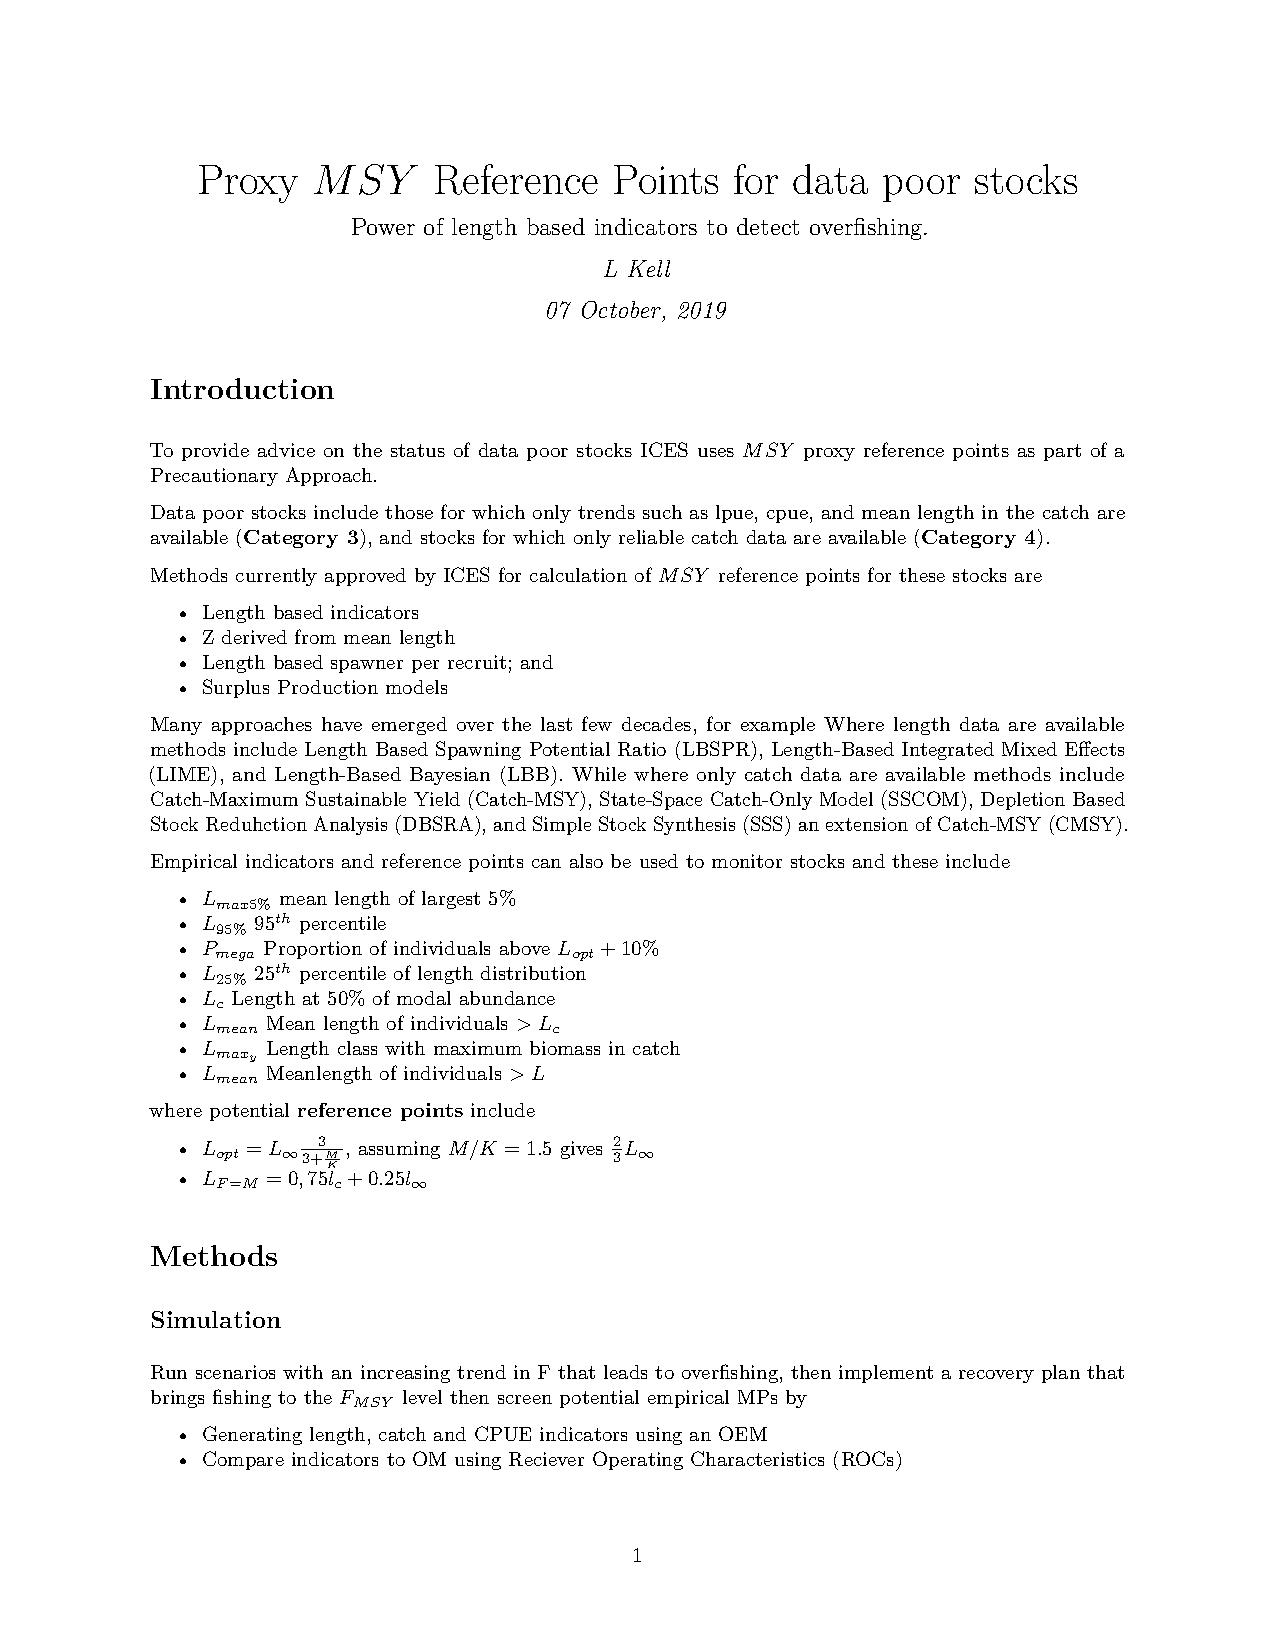
\includepdf[pages=1,pagecommand={},width=\textwidth]{../papers/roc/tex/roc.pdf}

\subsubsection{Pareto}

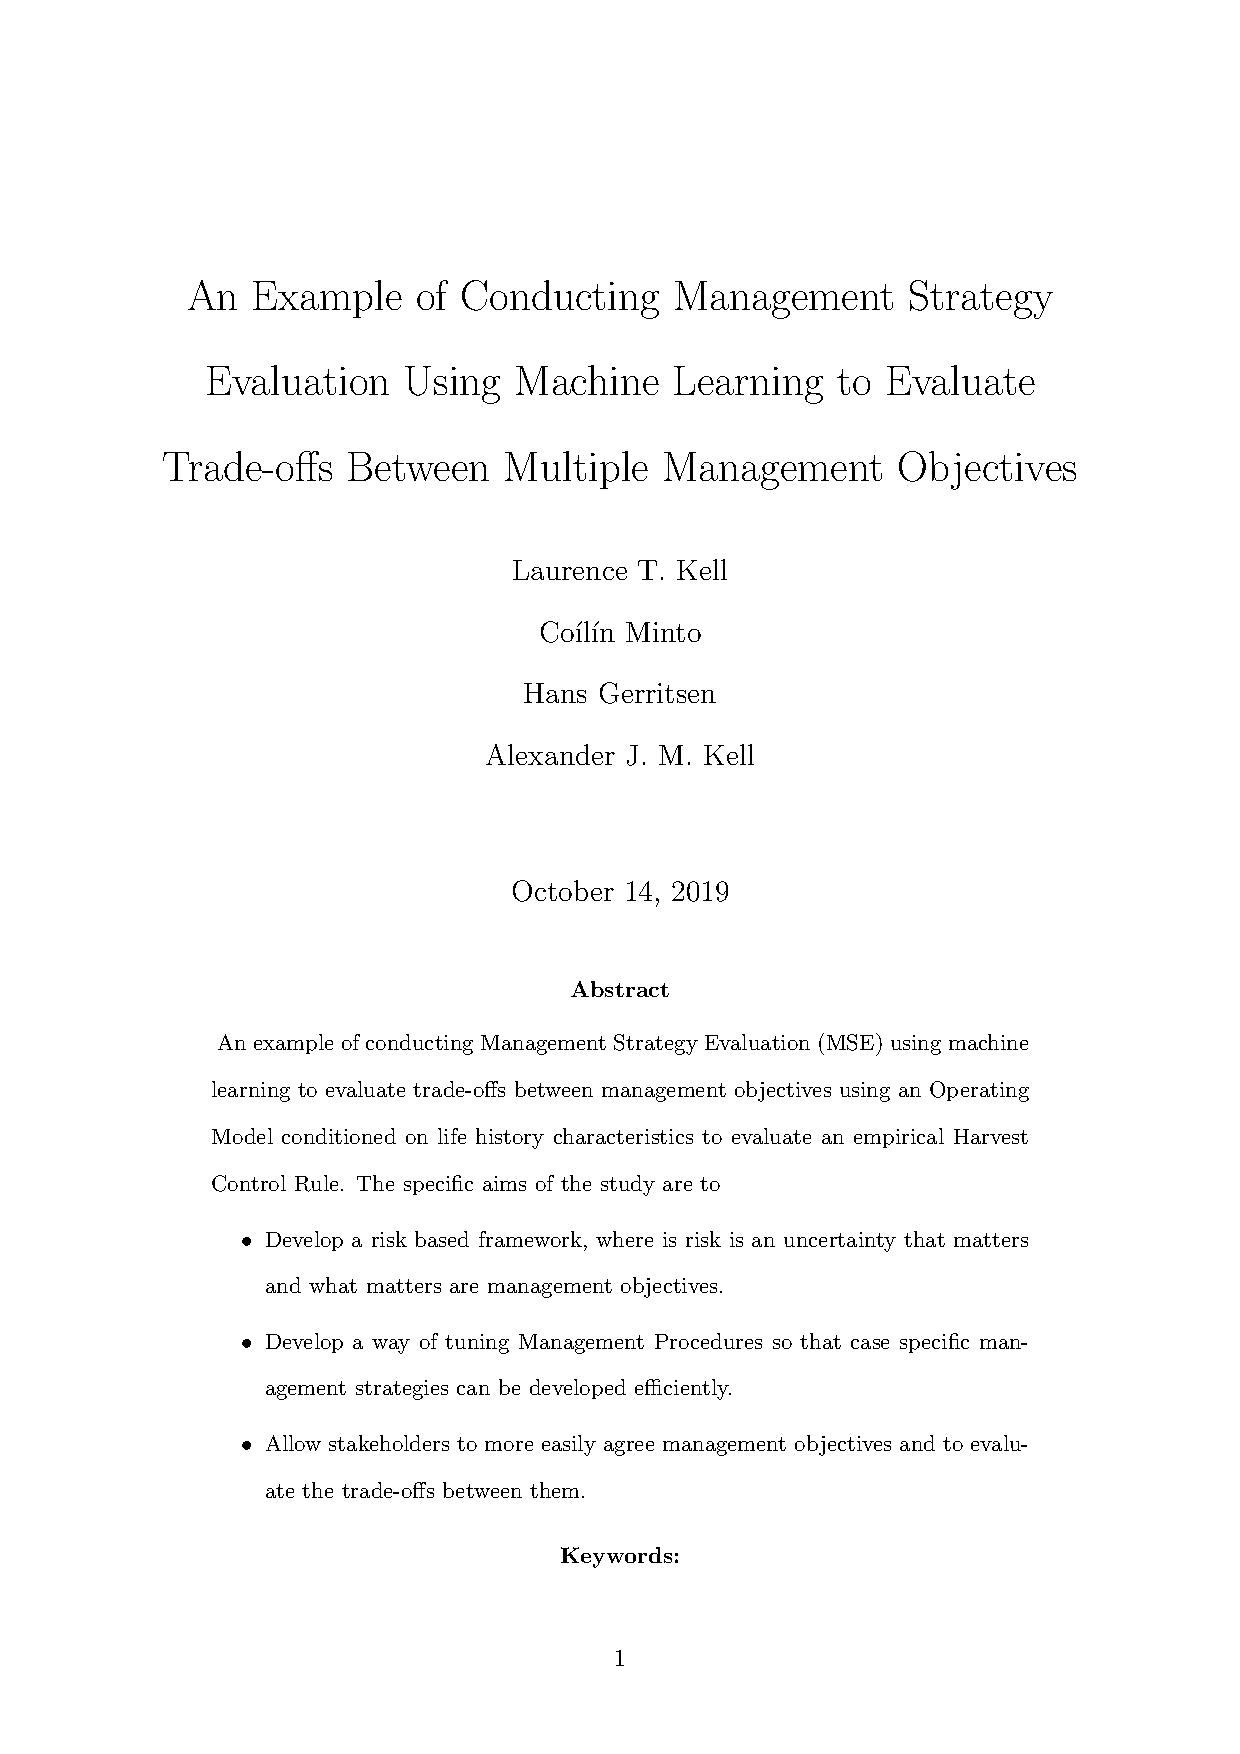
\includepdf[pages=1,pagecommand={},width=\textwidth]{../papers/pareto/tex/pareto.pdf}

\subsubsection{FLife}

\includepdf[pages=1,pagecommand={},width=\textwidth]{../papers/flife/tex/FLife.pdf}


\end{document}


%\newpage
%\begin{center}
%\section*{GMIT tax clearance certificate} 
%\end{center}
%\includepdf[pages=-]{GMIT_tax_clearance.pdf}

\end{document}












%%----------------
%% SANDBOX
%%----------------


\section{Reference Points}
\subsection{WKLIFE}


The specific Terms of Reference (ToRs) for this workshop are:
1. Collate necessary data and information for the stocks listed in Section 2 prior to the workshop.

2. Using methods provided by WKLIFE V, along with available data and expert judgement, propose precautionary and MSY proxies for each of the stocks
listed in Section 2.

3. Ascertain whether it is possible to define a desirable state of the stock assimilate to the state producing MSY; i.e. a state of the stock believed to produce high yields for a long period without a risk of stock depletion.

1. On similar basis, to explore whether it is possible to determine an undesirable state of the stock assimilate to a state where there is a risk of
very slow or no recovery towards desirable levels.

4. Assess the current situation of the stock relative to the desirable and undesirable states.
5. If necessary, update the guidelines provided by WKLIFE V.

6. During spring 2015 advisory process, if additional stocks are categorized as category 3 or 4, they should also be considered.

\subsection{Reference Points}

A variety of reference points and methods for deriving them are used for both data rich and poor stocks. Reference points may be derived as part of the stock assessment model, e.g. in a biomass dynamic model where MSY is a  function of the estimated parameters ($r$ and $K$), using an ad-hoc approach when using age methods such as VPA where assumptions about the stock recruitment relationship and future selection and biological parameters have to be made; or in a state space formulation such as SAM which actually estimates a prediction mechanism and reference points. 

In data poor situations a variety of statistical methods have been used to estimate stock status, productivity, fishing rates and reference points, for example using samples of length-composition  \citep{kokkalis2015limits,prince2015length}, age-composition  \citep{thorson2015catch}, fishery catch and fishing effort data  \citep{roa2015hierarchical}, abundance indices  \citep{needle2015using} or simple length-based reference points  \citep{cope2009length}.

In data poor cases identifying a link between a trigger point and stock status is the first step to being able to make management recommendations, e.g. using a harvest control rules (HCRs) where removals are linked to the current state of the resource as given by indicators or reference points  \citep{restrepo1999precautionary}.  \citep{cope2009length} proposed a way to do this for catch-based length proportions data poor stocks, using a decision tree and a risk assessmentcan, to provide advice within the context of existing management reference points. They also noted that a full examination of such HCRs requires a management strategy evaluation. 

In an MSE setting reference points are tuned, i.e. CCSBT provides a model-free example of a MP that is based on year-to-year changes and trends in empirical indicators (i.e. CPUE and fisheries independent indices); reference levels are then tuned to meet management objectives using MSE, where tuning refers to adjusting the parameters of the MP to try and achieve the stated objectives represented by the OM. Model-based MPs, for example those based on a stock assessment model, may include the estimation of MSY-based reference points, but the values of F, $F_{MSY}$ , B and $B_{MSY}$ from the OM do not need to be equivalent to their proxies in the MP (e.g. if a stock assessment models used in the MP is structually different from that used to condition the OM).

WKLIFE developed  operational  methods  for  setting  proxy reference  points for stocks  in  categories 3 (for which survey based assessments indicate trends) and 4 (for which reliable catch data are available).  These  methods  are noe being implemented  by  the ICES study group WKPROXY, ethods examined include length-based  indicators,  spawning  potential ratio (SPR), catch  and  cpue,  and  catch only based  methods.  

\end{document}


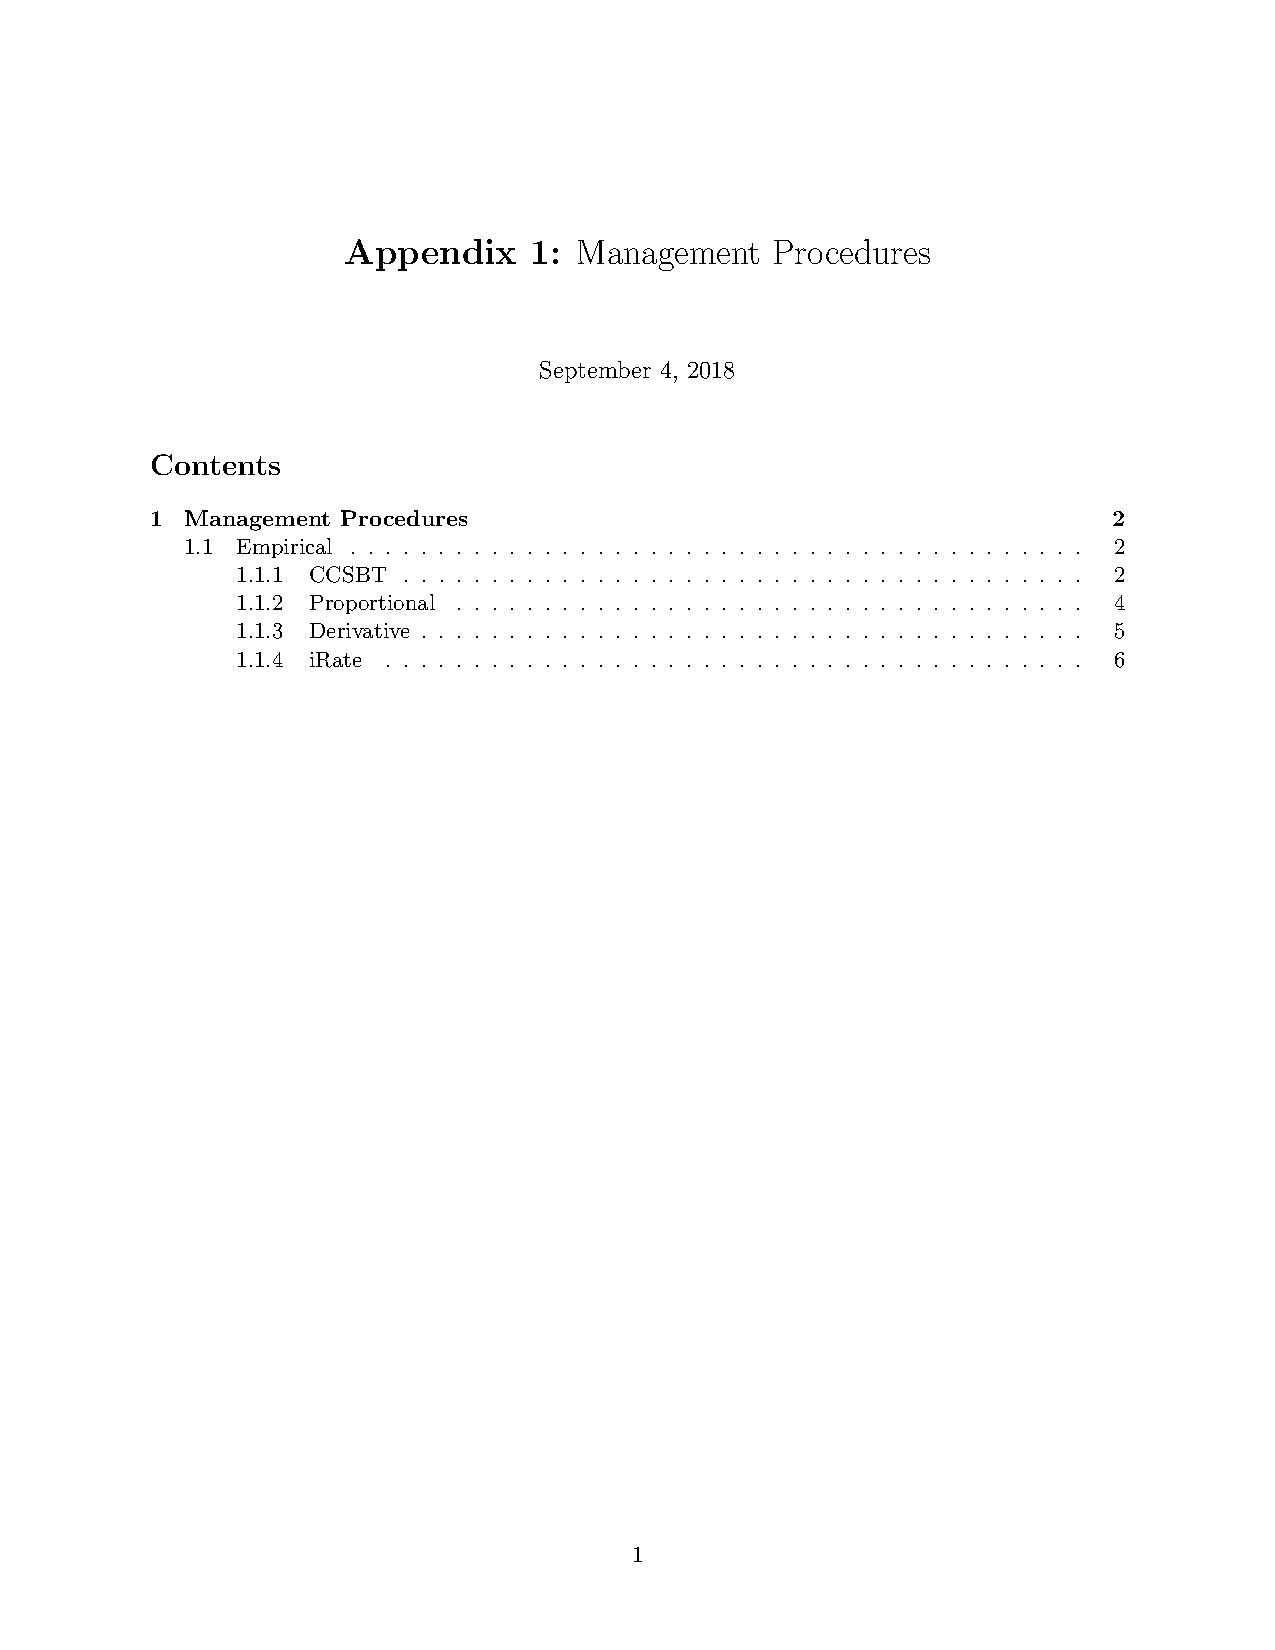
\includegraphics[width=12cm]{/home/laurie/Desktop/MEGAsync/projects/MI/mp.png}


%catch per unit effort from some fleets, total landings biomass, discards,survey, No age data, Some port sampling, observer and survey data, Very limited age data.

4.       Product/Service Specification

The Marine Institute requires research services on establishing MSY proxies for data-limited stocks 


General

The Marine Institute is tasked to implement the Marine Biodiversity Scheme which is part of the Seafood Development Operational Programme 2014-2020 funded under European Maritime Fisheries Fund (EMFF).  The objective of the Marine Biodiversity Scheme is to promote good fisheries and aquaculture management and protect biodiversity in marine habitats to support implementation of the CFP, and the Habitats and Birds Directives (Natura 2000) and the Marine Strategy Framework Directive.

The evaluation of biomass and fishing mortality against reference points for key stone species and/or species sensitive to the impacts of fishing has been identified as a priority action to be implemented under the Marine Biodiversity Scheme for the Marine Strategy Framework Directive (MSFD) and to support the implementation of the CFP. 

Many of the stocks which are caught by the Irish commercial fishing fleets are considered to be data-limited or are not assessed at all. This includes a number of key stone species (like sprat, gurnards, saithe, pollock, ling) and species sensitive to the impacts of fishing (like rays and skates, john dory, brill and turbot). For these stocks, the fishing mortality is unknown and MSY reference points are not established. This lack of quantifiable targets is an impediment to the implementation of the Common Fisheries Policy (CFP) as well as the Marine Strategy Framework Directive (MSFD).

There are a number of reasons why stocks are considered to be data limited: in some cases the available data is truly limited (e.g. non-TAC species or small stocks for which the value of the landings is small compared to the cost of sampling). In other cases there may be a substantial amount of data available, but not in a form that allows traditional analytical assessments of the status of the stock. 


\begin{center}
    \begin{tabular}{ | p{1.61cm} | p{1cm}  | p{3cm} | p{3cm}| p{3cm}|}
    \hline
    Species   & TAC & Commercial Catch & Data & Comments \\ \hline

    Sprat     & No  &Targeted species for small fleet & Poor; mainly landings weights  & Key-stone prey fish\\ \hline
    Gurnards  & No  &Nearly 100\% discarded  & Reasonable discard and survey data. No age data & Key-stone prey – widely distributed and abundant\\ \hline
    Saithe
    Pollock
    Ling      & Yes &Mixed fishery  & Some port sampling, observer and survey data. Very limited age data & Key-stone predator\\ \hline
    Rays 
    Skates    & Yes &Targeted and mixed fishery  & Some port sampling, observer and survey data. No age data & Sensitive species – slow reproduction\\ \hline
    John Dory & No  &Mixed fishery but can be targeted to an extent  & Some port sampling, observer and survey data. No age data & Sensitive species – valuable non-TAC species (not protected by fisheries management)\\ \hline
    Turbot
    Brill     & No  &Mixed fishery but can be targeted to an extent  & Some port sampling, observer and survey data. Very limited age data & Sensitive species – valuable non-TAC species (not protected by fisheries management)\\ \hline
\end{tabular}
\end{center}


Most of these species are caught in a mixed fishery. Some species cannot be aged and for others the value of the landings is too low to justify a sampling programme to support age-based assessments. Nevertheless, apart from catch data, some additional data exists for most of these stocks (e.g. commercial LPUE and survey data). The project will evaluate whether including these additional sources of data improves or actually deteriorates our understanding of the state of the stock, compared to the information that is available from the time series of landings or catches alone. 
For other stocks, that are almost data-rich but for which no appropriate assessment models exists, the project will develop assessment methods that make optimal use of the available data. Each data source will be assessed for bias and precision and the contribution it makes to the assessment model.

There are also a large number of stocks in the ICES area for which reliable analytical assessments exist and for which the state of the stock is well known (e.g. Celtic Sea haddock, Irish Sea Nephrops). These stocks can be used to simulate data-limited situations and evaluate the performance of data-limited assessment models. In addition to this, models will be tested with fully simulated fish stocks and fisheries.

Simulated fish stocks and fisheries will also be used for a cost-benefit analysis of including various sources of data. This will answer the question of when the cost of collecting additional data would offset the yield and conservation benefits. For example: how many years would it take for an ageing programme to be financially viable under a range of stock scenarios. 

The overall aim of the project is to develop and test a range of assessment models and methods to establish MSY reference points (or proxy MSY reference points) across the spectrum of data-limited stocks. 

There is a requirement for the following research services over a 24 months period between May 2017 and April 2019:

Task 1: Stock prioritisation
A number of example stocks have been identified above. The final list of stocks will be prioritised using criteria like: economic value of the stock; importance of the species to the ecosystem (key-stone species); sensitivity to the impacts of fishing; available data.

Task 2: Data collation (to run in parallel with other tasks)	
The project relies on existing data sets, however these data need to be collated in a usable form. Most datasets are available from the Marine Institute, or are publicly available, but others may only exist in other European labs/agencies.

Task 3: Method and simulation framework development and implementation
A number of data-limited methods exist. In order to compare the performance of these methods it would be useful to implement them all in the same framework, e.g. R. New methods may also be developed in the same framework.

Task 4: Method performance appraisal
Develop set of diagnostics that can be applied across range of models. Also assess the stability of the model, sensitivity to assumptions and bias in the advised catch.

Task 5: Reference point comparisons (across candidate methods)
Once reference points have been identified, their performance should be evaluated through simple management strategy evaluations.

Task 6: Liaison with Marine Institute
The service provider is expected to meet on a regular basis with Marine Institute staff involved in the project:
Monthly update meetings at the Marine Institute premises in Oranmore Galway with researcher providing the research services, 
6-monthly progress reports and meetings at the Marine Institute with the researcher providing the research services and contract manager. 

Task 7: Linkage with other projects
The service provider is required to link research output to the following projects: 

The International Council of the Exploration of the Sea (ICES) is in the process of developing methods to identify MSY proxy reference points for data-limited stocks (WKLIFE and WKPROXY series of workshops). The service provider is required to contribute to this process by proposing and testing new assessment models and methods of establishing reference points and will be expected to attend up to 4 one-week meetings at ICES headquarters in Copenhagen. However there are key differences with the ICES approach: 
This research contract will include stocks not currently assessed by ICES;
this research contract will focus on the available data for each stock first and on the methods second; the ICES approach focuses on the methods first and then applies a limited number of methods to a large number of stocks.
Marine Institute research and development on data poor stocks which includes the biology, stock dynamics and Management Strategy Evaluation (MSE) for Pollock.  It is expected that the service provider will collaborate closely with the team developing assessment methods for the pollock stock.
Galway Mayo Institute of Technology MIT had been awarded a Cullen fellowship for a PhD project on management strategy evaluation for monkfish. It is expected that the Cullen PhD and service provider will closely collaborate on tasks like data collation, assessment model implementation, simulation model development and management strategy evaluation. 

Expected outputs: 
A collection of existing and new assessment models for data-limited stocks, all implemented in the same framework (e.g. R) with a set of diagnostic tools that can be applied to all models.
A set of proposed reference points for a range of stocks with associated management strategy evaluations to contribute to sustainable management of these stocks.
Working documents describing the methods and findings to relevant ICES groups (e.g WGCSE; WKPROXY).
Publication(s) in peer-reviewed journals on new methods/tools/evaluations.

Minimum Qualifications/Education/Experience: 
The researcher providing the research services must meet the following minimum requirements:
A PhD in fisheries science or a related discipline, or at least 2 years of work experience involving stock assessment.
A strong quantitative background with demonstrated experience in statistical modelling and programming (e.g., R programming language).

\section{Reference Points}
\subsection{WKLIFE}


The specific Terms of Reference (ToRs) for this workshop are:
1. Collate necessary data and information for the stocks listed in Section 2 prior to the workshop.

2. Using methods provided by WKLIFE V, along with available data and expert judgement, propose precautionary and MSY proxies for each of the stocks
listed in Section 2.

3. Ascertain whether it is possible to define a desirable state of the stock assimilate to the state producing MSY; i.e. a state of the stock believed to produce high yields for a long period without a risk of stock depletion.

1. On similar basis, to explore whether it is possible to determine an undesirable state of the stock assimilate to a state where there is a risk of
very slow or no recovery towards desirable levels.

4. Assess the current situation of the stock relative to the desirable and undesirable states.
5. If necessary, update the guidelines provided by WKLIFE V.

6. During spring 2015 advisory process, if additional stocks are categorized as category 3 or 4, they should also be considered.

\subsection{Reference Points}

A variety of reference points and methods for deriving them are used for both data rich and poor stocks. Reference points may be derived as part of the stock assessment model, e.g. in a biomass dynamic model where MSY is a  function of the estimated parameters ($r$ and $K$), using an ad-hoc approach when using age methodsl such as VPA where assumptions about the stock recruitment relationship and future selection and biological parameters have to be made; or in a state space formulation such as SAM which actually estimates a prediction mechanism and reference points. 


In a data poor situation a variety of statistical methods have been used to estimate stock status, productivity, fishing rates and reference points, for example using samples of length-composition  \citep{kokkalis2015limits,prince2015length}, age-composition  \citep{thorson2015catch}, fishery catch and fishing effort data  \citep{roa2015hierarchical}, abundance indices  \citep{needle2015using} or simple length-based reference points  \citep{cope2009length}.

In data poor cases identifying a link between a trigger point and stock status is the first step to being able to make management recommendations, e.g. using a harvest control rules (HCRs) to link removals to the current state of the resource as given by indicators or reference points  \citep{restrepo1999precautionary}. 

 \citep{cope2009length} proposed a decision tree and a risk assessment suggesting ways in which catch-based length proportions can be used to provide advice regarding harvest regulation within the context of existing management RPs. There noted that a full examination of such HCRs requires a management strategy evaluation. 


In an MSE setting reference points are tuned, i.e. CCSBT provides a model-free example of a MP that is based on year-to-year changes and trends in empirical indicators (i.e. CPUE and fisheries independent indices); reference levels are then tuned to meet management objectives using MSE, where tuning refers to adjusting the parameters of the MP to try and achieve the stated objectives represented by the OM. Model-based MPs, for example those based on a stock assessment model, may include the estimation of MSY-based reference points, but the values of F, $F_{MSY}$ , B and $B_{MSY}$ from the OM do not need to be equivalent to their proxies in the MP (e.g. if a stock assessment models used in the MP is structually different from that used to condition the OM).



Generally, TRPs and LRPs are divided into two categories: fishing mortality-based (F-based) and biomass-based
(B-based). For many decades, reference points have most often been tied to maximum sustainable yield (MSY),
defi ned as the largest average catch that can be taken continuously from a stock under existing environmental
conditions. There are two related reference points: FMSY is the fi shing mortality rate that eventually results in the
largest yield on average (MSY); BMSY is the corresponding average stock size.
One key question that managers face is whether to use F-based and/or B-based reference points when setting
targets and limits. Oftentimes, the answer is to use both, because F can be directly managed while B is the
critical point to control from an ecological perspective.2
 B-based reference points are also often easier for
managers and stakeholders to understand, because biomass is usually expressed as an absolute number that
relates physically to the quantity of fi sh in the water, whereas F is a mortality rate that is intangible and cannot be
directly observed.
Although MSY is an appropriate basis for reference points in many cases, there are situations in which MSY
should not be used, either because it cannot be robustly estimated or because the management objective
is unrelated to MSY. In those cases, many other candidate reference points exist to choose from, each with 
their own strengths and weaknesses. (See Table 1.) Most reference points are calculated from the results of
stock assessments, but it is also possible to set empirical, or data-based, reference points that can be directly
measured; for example, those related to catch per unit e ort (CPUE).
Guidelines for developing and using target and limit reference points are outlined in the United Nations Fish
Stocks Agreement (UNFSA) and the Food and Agriculture Organization Code of Conduct for Responsible
Fisheries. (See below.) The Marine Stewardship Council also calls on fi sheries to be managed with target and
limit reference points in order to be certifi ed as sustainable. That guidance can help fi sheries choose among the
many candidate reference points


WKLIFE  V  developed  operational  methods  for  setting  reference  point  proxies  for stocks  in  categories  3  and  4.  These  meth
ods  will  be  implemented  by  ICES scientists with  expert  knowledge  of  the  stocks  and  fisheries  in
  a  subsequent  ICES  meeting [WKProxy].  Several  methodological  approaches  to
  data-limited  stock  assessment  were reviewed and applied to both data
-limited (e.g. Nephrops  FUs  28-29  by  sex,  sea bass  in  the  Bay  of  Biscay,  sole  in  the  Bay  of  Biscay)  and  data-rich
  case  studies  (e.g. Northern hake) to evaluated strengths and weaknesses of each approach for applica-
tion  to  the  ICES  DLS  advisory  framework   (ICES,  2012)
.  The  reviewed  approaches  included  
length-based  indicators  and  reference  points,  spawning  potential  ratio (SPR),  
catch  and  cpue
-based  methods,  and  catch
-based  methods.  The  prospects  of managing other crustaceans and molluscs using minimum legal size was also evaluated.  The  methods  most  suitable  to  the  data  and  expertise  available  were  identified  for each of the requested stocks on the western shelf for ICES  WKProxy.

\end{document}

4.       Product/Service Specification

The Marine Institute requires research services on establishing MSY proxies for data-limited stocks 

General

The Marine Institute is tasked to implement the Marine Biodiversity Scheme which is part of the Seafood Development Operational Programme 2014-2020 funded under European Maritime Fisheries Fund (EMFF).  The objective of the Marine Biodiversity Scheme is to promote good fisheries and aquaculture management and protect biodiversity in marine habitats to support implementation of the CFP, and the Habitats and Birds Directives (Natura 2000) and the Marine Strategy Framework Directive.

The evaluation of biomass and fishing mortality against reference points for key stone species and/or species sensitive to the impacts of fishing has been identified as a priority action to be implemented under the Marine Biodiversity Scheme for the Marine Strategy Framework Directive (MSFD) and to support the implementation of the CFP. 

Many of the stocks which are caught by the Irish commercial fishing fleets are considered to be data-limited or are not assessed at all. This includes a number of key stone species (like sprat, gurnards, saithe, pollock, ling) and species sensitive to the impacts of fishing (like rays and skates, john dory, brill and turbot). For these stocks, the fishing mortality is unknown and MSY reference points are not established. This lack of quantifiable targets is an impediment to the implementation of the Common Fisheries Policy (CFP) as well as the Marine Strategy Framework Directive (MSFD).

There are a number of reasons why stocks are considered to be data limited: in some cases the available data is truly limited (e.g. non-TAC species or small stocks for which the value of the landings is small compared to the cost of sampling). In other cases there may be a substantial amount of data available, but not in a form that allows traditional analytical assessments of the status of the stock. 


\begin{center}
    \begin{tabular}{ | p{1.61cm} | p{1cm}  | p{3cm} | p{3cm}| p{3cm}|}
    \hline
    Species   & TAC & Commercial Catch & Data & Comments \\ \hline

    Sprat     & No  &Targeted species for small fleet & Poor; mainly landings weights  & Key-stone prey fish\\ \hline
    Gurnards  & No  &Nearly 100\% discarded  & Reasonable discard and survey data. No age data & Key-stone prey – widely distributed and abundant\\ \hline
    Saithe
    Pollock
    Ling      & Yes &Mixed fishery  & Some port sampling, observer and survey data. Very limited age data & Key-stone predator\\ \hline
    Rays 
    Skates    & Yes &Targeted and mixed fishery  & Some port sampling, observer and survey data. No age data & Sensitive species – slow reproduction\\ \hline
    John Dory & No  &Mixed fishery but can be targeted to an extent  & Some port sampling, observer and survey data. No age data & Sensitive species – valuable non-TAC species (not protected by fisheries management)\\ \hline
    Turbot
    Brill     & No  &Mixed fishery but can be targeted to an extent  & Some port sampling, observer and survey data. Very limited age data & Sensitive species – valuable non-TAC species (not protected by fisheries management)\\ \hline
\end{tabular}
\end{center}


Most of these species are caught in a mixed fishery. Some species cannot be aged and for others the value of the landings is too low to justify a sampling programme to support age-based assessments. Nevertheless, apart from catch data, some additional data exists for most of these stocks (e.g. commercial LPUE and survey data). The project will evaluate whether including these additional sources of data improves or actually deteriorates our understanding of the state of the stock, compared to the information that is available from the time series of landings or catches alone. 
For other stocks, that are almost data-rich but for which no appropriate assessment models exists, the project will develop assessment methods that make optimal use of the available data. Each data source will be assessed for bias and precision and the contribution it makes to the assessment model.

There are also a large number of stocks in the ICES area for which reliable analytical assessments exist and for which the state of the stock is well known (e.g. Celtic Sea haddock, Irish Sea Nephrops). These stocks can be used to simulate data-limited situations and evaluate the performance of data-limited assessment models. In addition to this, models will be tested with fully simulated fish stocks and fisheries.

Simulated fish stocks and fisheries will also be used for a cost-benefit analysis of including various sources of data. This will answer the question of when the cost of collecting additional data would offset the yield and conservation benefits. For example: how many years would it take for an ageing programme to be financially viable under a range of stock scenarios. 

The overall aim of the project is to develop and test a range of assessment models and methods to establish MSY reference points (or proxy MSY reference points) across the spectrum of data-limited stocks. 

There is a requirement for the following research services over a 24 months period between May 2017 and April 2019:

Task 1: Stock prioritisation
A number of example stocks have been identified above. The final list of stocks will be prioritised using criteria like: economic value of the stock; importance of the species to the ecosystem (key-stone species); sensitivity to the impacts of fishing; available data.

Task 2: Data collation (to run in parallel with other tasks)	
The project relies on existing data sets, however these data need to be collated in a usable form. Most datasets are available from the Marine Institute, or are publicly available, but others may only exist in other European labs/agencies.

Task 3: Method and simulation framework development and implementation
A number of data-limited methods exist. In order to compare the performance of these methods it would be useful to implement them all in the same framework, e.g. R. New methods may also be developed in the same framework.

Task 4: Method performance appraisal
Develop set of diagnostics that can be applied across range of models. Also assess the stability of the model, sensitivity to assumptions and bias in the advised catch.

Task 5: Reference point comparisons (across candidate methods)
Once reference points have been identified, their performance should be evaluated through simple management strategy evaluations.

Task 6: Liaison with Marine Institute
The service provider is expected to meet on a regular basis with Marine Institute staff involved in the project:
Monthly update meetings at the Marine Institute premises in Oranmore Galway with researcher providing the research services, 
6-monthly progress reports and meetings at the Marine Institute with the researcher providing the research services and contract manager. 

Task 7: Linkage with other projects
The service provider is required to link research output to the following projects: 

The International Council of the Exploration of the Sea (ICES) is in the process of developing methods to identify MSY proxy reference points for data-limited stocks (WKLIFE and WKPROXY series of workshops). The service provider is required to contribute to this process by proposing and testing new assessment models and methods of establishing reference points and will be expected to attend up to 4 one-week meetings at ICES headquarters in Copenhagen. However there are key differences with the ICES approach: 
This research contract will include stocks not currently assessed by ICES;
this research contract will focus on the available data for each stock first and on the methods second; the ICES approach focuses on the methods first and then applies a limited number of methods to a large number of stocks.
Marine Institute research and development on data poor stocks which includes the biology, stock dynamics and Management Strategy Evaluation (MSE) for Pollock.  It is expected that the service provider will collaborate closely with the team developing assessment methods for the pollock stock.
Galway Mayo Institute of Technology MIT had been awarded a Cullen fellowship for a PhD project on management strategy evaluation for monkfish. It is expected that the Cullen PhD and service provider will closely collaborate on tasks like data collation, assessment model implementation, simulation model development and management strategy evaluation. 

Expected outputs: 
A collection of existing and new assessment models for data-limited stocks, all implemented in the same framework (e.g. R) with a set of diagnostic tools that can be applied to all models.

A set of proposed reference points for a range of stocks with associated management strategy evaluations to contribute to sustainable management of these stocks.

Working documents describing the methods and findings to relevant ICES groups (e.g WGCSE; WKPROXY).
Publication(s) in peer-reviewed journals on new methods/tools/evaluations.

Minimum Qualifications/Education/Experience: 
The researcher providing the research services must meet the following minimum requirements:
A PhD in fisheries science or a related discipline, or at least 2 years of work experience involving stock assessment.
A strong quantitative background with demonstrated experience in statistical modelling and programming (e.g., R programming language).


\begin{table}
	\caption{Levels of NLP}
	\begin{center}
	\begin{tabular}{l p{.5cm} p{4cm} p{.5cm} l}
		\hline\noalign{\smallskip}
		Level & & Problems & & Methods/KB \\
		\noalign{\smallskip} 
		\hline
		\noalign{\smallskip} 
			Lexical
			& &
			Part of speech (POS) tagging
			& &
			\parbox[t]{5cm}{
			\raggedright
				Part of speech tagger\break
				Corpora: WSJ, Brown Corpus\\
			}
			 \\ \\
			Syntactic
			& &
			Generation of parse-trees representing syntactic structure of
				sentence
			& &
			\parbox[t]{5cm}{
			\raggedright
				Probabilistic parsers\break
				Corpora: WSJ, Brown Corpus\\
			}				
			\\ \\
			Semantic
			& &
			Reference resolution; Context modeling; Word-Sense Disambiguation
			& &
			\parbox[t]{5cm}{
			\raggedright
				Semantic parsers, WSD Classifiers;\break
				Corpora: FrameNet, SENSEVAL\\
			}
			\\ \\
			Pragmatic
			& &
			Goal, content or topic of a text or discourse; Anaphora Resolution
			& &
			\parbox[t]{5cm}{
			\raggedright
				Text summarization;\break
				Text categorization\break
				Corpora: WordNet, SummBank
			}
			\\
		\hline
	\end{tabular}
\end{center}
\label{tab:nlplevels}
\end{table}

\end{document}
